\paragraph{1. Permission toevoegen}
Om toegang te krijgen tot de sensoren moet er een user-permission toegevoegd worden aan het 
AndroidManifest.xml bestand.
\begin{minted}{xml}
<uses-permission android:name=
    "android.permission.ACCESS_FINE_LOCATION" />
\end{minted}

\paragraph{2. SensorManager initialiseren}
Om toegang te krijgen tot de sensoren moet er een instantie van de SensorManager klasse aangemaakt worden.
\begin{minted}{kotlin}
private lateinit var sensorManager: SensorManager
private var accelerometer: Sensor? = null
private var gyroscope: Sensor? = null
\end{minted}
Daarna worden de variabelen met behulp van de sensorManager gelinkt aan een sensor met de onCreate methode.
\begin{minted}{kotlin}
override fun onCreate(savedInstanceState: Bundle?) {
    super.onCreate(savedInstanceState)
    setContentView(R.layout.activity_main)

    sensorManager = getSystemService(Context.SENSOR_SERVICE) as SensorManager
    accelerometer = sensorManager.getDefaultSensor(Sensor.TYPE_ACCELEROMETER)
    gyroscope = sensorManager.getDefaultSensor(Sensor.TYPE_GYROSCOPE)
}
\end{minted}

\paragraph{3. SensorEventListener initialiseren}
Daarna wordt de SensorEventListener aangemaakt, hiervoor wordt de onSensorChanged methode gebruikt.
\begin{minted}{kotlin}
private val sensorEventListener = object : SensorEventListener {
    override fun onSensorChanged(event: SensorEvent) {
        if (event.sensor.type == Sensor.TYPE_ACCELEROMETER) {
            val x = event.values[0]
            val y = event.values[1]
            val z = event.values[2]
            // Doe iets met de accelerometerwaarden (x, y, z)
        } else if (event.sensor.type == Sensor.TYPE_GYROSCOPE) {
            val x = event.values[0]
            val y = event.values[1]
            val z = event.values[2]
            // Doe iets met de gyroscoopwaarden (x, y, z)
        }
    }

    override fun onAccuracyChanged(sensor: Sensor?, accuracy: Int) {
        return // Niet nodig bij dit onderzoek
    }
}
\end{minted}
Nu kan de data van de sensoren worden uitgelezen in de onSensorChanged methode.
\begin{minted}{kotlin}
fetchButton.setOnClickListener {
    sensorManager.registerListener(
        sensorEventListener,
        sensor, // Veranderen door gyroscope of accelerometer
        SensorManager.SENSOR_DELAY_NORMAL
    )
}
\end{minted}

\paragraph{4. Applicatie maken}
Met deze informatie wordt een applicatie opgebouwd die de data van sensoren 
ophaalt. De applicatie bestaat uit twee \textbf{TextView} componenten voor de data van de 
accelerometer en gyroscoop en tot slot twee \textbf{Button} componenten om de data op te halen. 
Als de knoppen ingedrukt worden, dan worden de setOnClickListener methodes aangeroepen.
In de onSensorChanged methode wordt de data van de sensoren opgehaald en in de TextViews
geplaatst.
\begin{figure}[H]
    \centering
    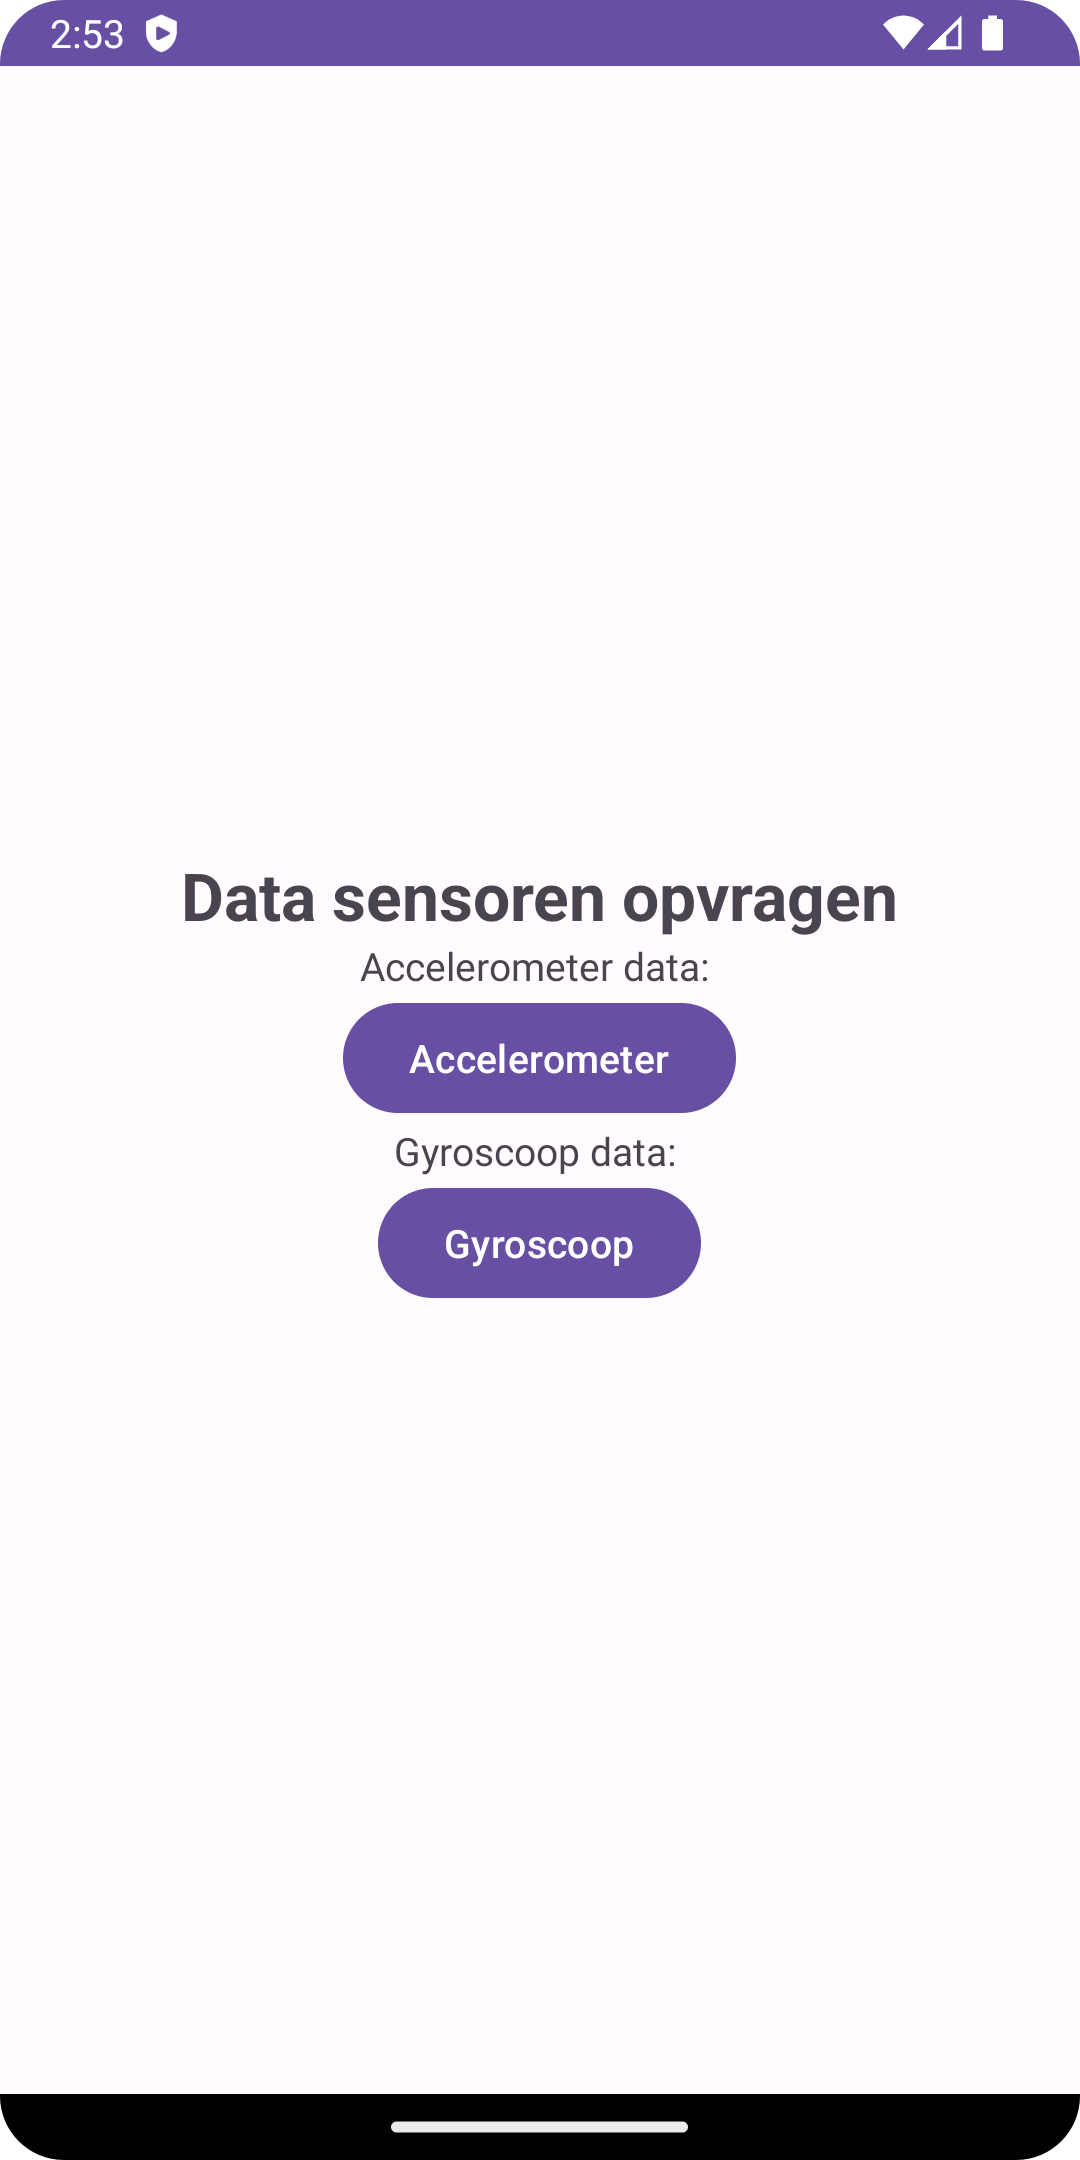
\includegraphics[height=0.5\textheight]{sensoren_layoutnative.png}
    \caption{Layout van applicatie voor data van sensoren op te halen bij Android.}
\end{figure}
